\documentclass [14pt,xcolor=x11names,t,pstricks] {beamer} 

\input{Cmd}

\title[Schéma de Lewis]{Formation de liaison chimiques}
\date{}

\titlegraphic{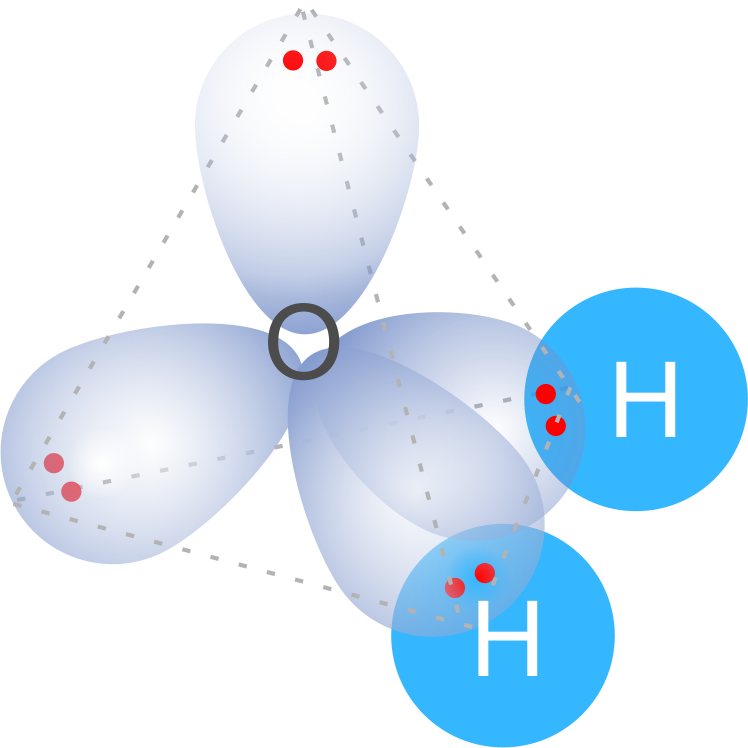
\includegraphics[height=4.0cm]{Ressources/h2o_sp3.png}}




\begin{document}
\begin{frame}
\maketitle
\end{frame}



%%%%%%%%%%%%%%%%%%%%%%%%%%%%%%%%%%%%%

\begin{frame}
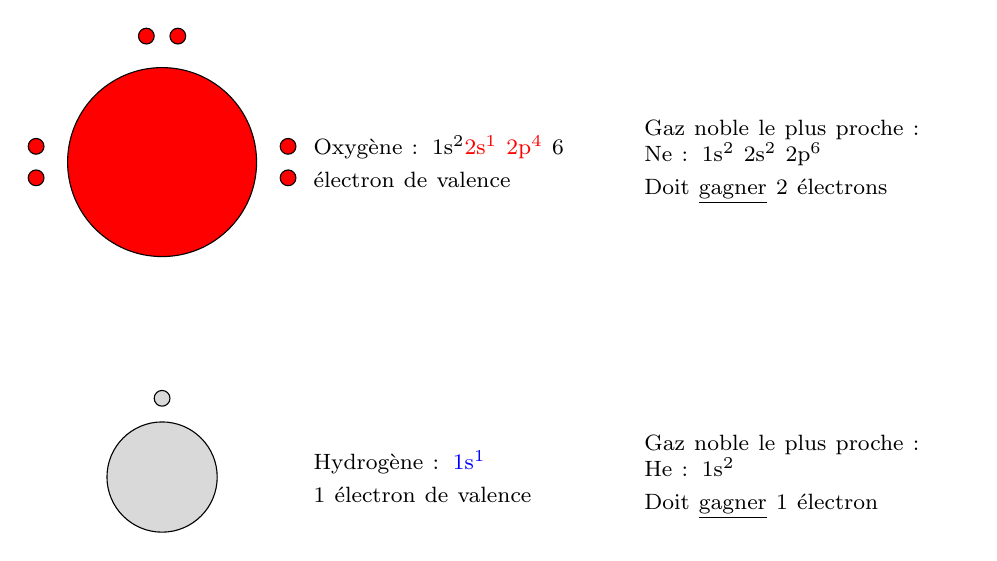
\begin{tikzpicture}
    \fill[red,draw=black] (0,0) circle(1.2);
    \foreach \k in {-1.6,1.6} {
        \fill[red,draw=black] (\k,-.2) circle(.1);
        \fill[red,draw=black] (\k,.2) circle(.1);
    }
    \fill[red,draw=black] (-.2,1.6) circle(.1);
    \fill[red,draw=black] (.2,1.6) circle(.1);
    
    \fill[gray!30,draw=black] (0,-4) circle(.7);
    \fill[gray!30,draw=black] (0,-3) circle(.1);
    \pause
    \node[right, text width = 4cm] at (1.8,-4){\footnotesize Hydrogène : \textcolor{blue}{1s$^1$}\\ 1 électron de valence};
    \node[right, text width = 3.5cm] at (1.8,0){\footnotesize Oxygène : 1s$^2$\textcolor{red}{2s$^1$ 2p$^4$} 6 électron de valence};
    \pause
    \node[right, text width = 4cm] at (6,-4){\footnotesize  Gaz noble le plus proche : He : 1s$^2$ \\ Doit \underline{gagner} 1 électron};
    \node[right, text width = 4cm] at (6,0){\footnotesize Gaz noble le plus proche : Ne : 1s$^2$ 2s$^2$ 2p$^6$ \\ Doit \underline{gagner} 2 électrons};
\end{tikzpicture} 
\end{frame}

\begin{frame}
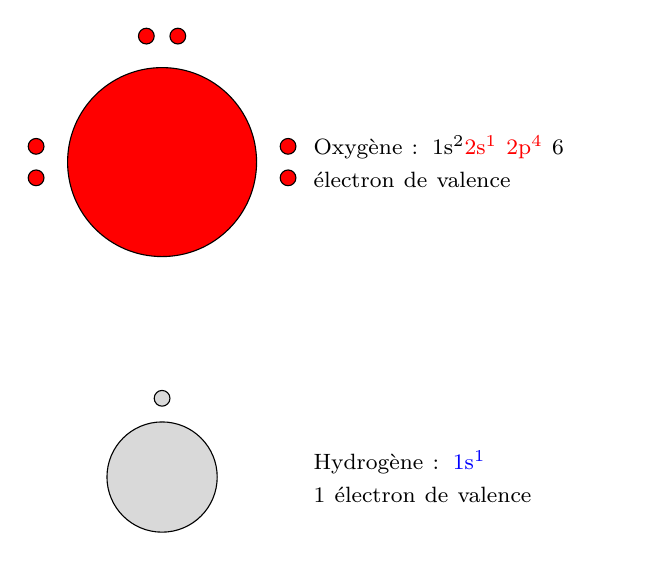
\begin{tikzpicture}
    \fill[red,draw=black] (0,0) circle(1.2);
    \foreach \k in {-1.6,1.6} {
        \fill[red,draw=black] (\k,-.2) circle(.1);
        \fill[red,draw=black] (\k,.2) circle(.1);
    }
    \fill[red,draw=black] (-.2,1.6) circle(.1);
    \fill[red,draw=black] (.2,1.6) circle(.1);
    
    \fill[gray!30,draw=black] (0,-4) circle(.7);
    \fill[gray!30,draw=black] (0,-3) circle(.1);
    
    \node[right, text width = 4cm] at (1.8,-4){\footnotesize Hydrogène : \textcolor{blue}{1s$^1$}\\ 1 électron de valence};
    \node[right, text width = 3.5cm] at (1.8,0){\footnotesize Oxygène : 1s$^2$\textcolor{red}{2s$^1$ 2p$^4$} 6 électron de valence};
\end{tikzpicture}


\centering\colorbox{orange!10}{\begin{minipage}{.8\textwidth}
    \begin{center}\textbf{Comment expliquer la formation de la molécule d'eau ?}
    \end{center}
    \end{minipage}}
\end{frame}

\begin{frame}
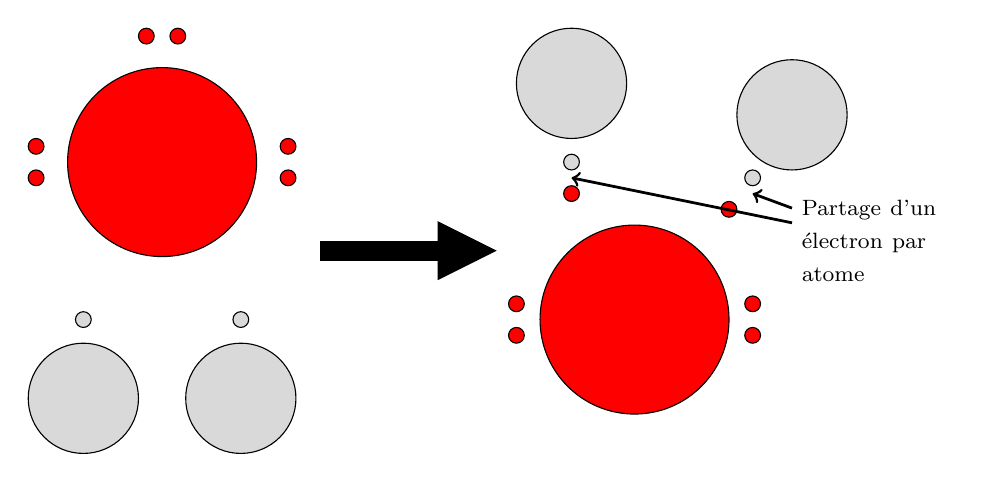
\begin{tikzpicture}
    \fill[red,draw=black] (0,0) circle(1.2);
    \foreach \k in {-1.6,1.6} {
        \fill[red,draw=black] (\k,-.2) circle(.1);
        \fill[red,draw=black] (\k,.2) circle(.1);
    }
    \fill[red,draw=black] (-.2,1.6) circle(.1);
    \fill[red,draw=black] (.2,1.6) circle(.1);
    
    \fill[gray!30,draw=black] (-1,-3) circle(.7);
    \fill[gray!30,draw=black] (-1,-2) circle(.1);

    \fill[gray!30,draw=black] (1,-3) circle(.7);
    \fill[gray!30,draw=black] (1,-2) circle(.1);
    
    \pause %Partie droite
    
    \fill[black] (2,-1.25)--(2,-1)--(4,-1)--(4,-1.25)--cycle;
    \fill[black] (3.5,-1.5)--(3.5,-.75)--(4.25,-1.125)--cycle;

    \fill[red,draw=black] (6,-2) circle(1.2);
    \fill[red,draw=black] (4.5,-1.8) circle(.1);
    \fill[red,draw=black] (4.5,-2.2) circle(.1);
    \fill[red,draw=black] (7.5,-1.8) circle(.1);
    \fill[red,draw=black] (7.5,-2.2) circle(.1);
    
    \fill[red,draw=black] (5.2,-.4) circle(.1);
    \fill[red,draw=black] (7.2,-.6) circle(.1);
    
    \fill[gray!30,draw=black] (5.2,1) circle(.7);
    \fill[gray!30,draw=black] (5.2,0) circle(.1);

    \fill[gray!30,draw=black] (8,.6) circle(.7);
    \fill[gray!30,draw=black] (7.5,-.2) circle(.1);

    \pause
    \node[right,text width = 2 cm] (E) at (8,-1) {\footnotesize Partage d'un électron par atome};
    \draw[->,line width = 1pt] (E) to (5.2,-.2);
    \draw[->,line width = 1pt] (E) to (7.5,-.4);
\end{tikzpicture}
\pause
   \centering\colorbox{green!10}{\begin{minipage}{.8\textwidth}
    \begin{center}\textbf{Le partage d'électron permet de stabiliser les atomes}
    \end{center}
    \end{minipage}}

\end{frame}
\begin{frame}{Règles du duet et de l'octet}
    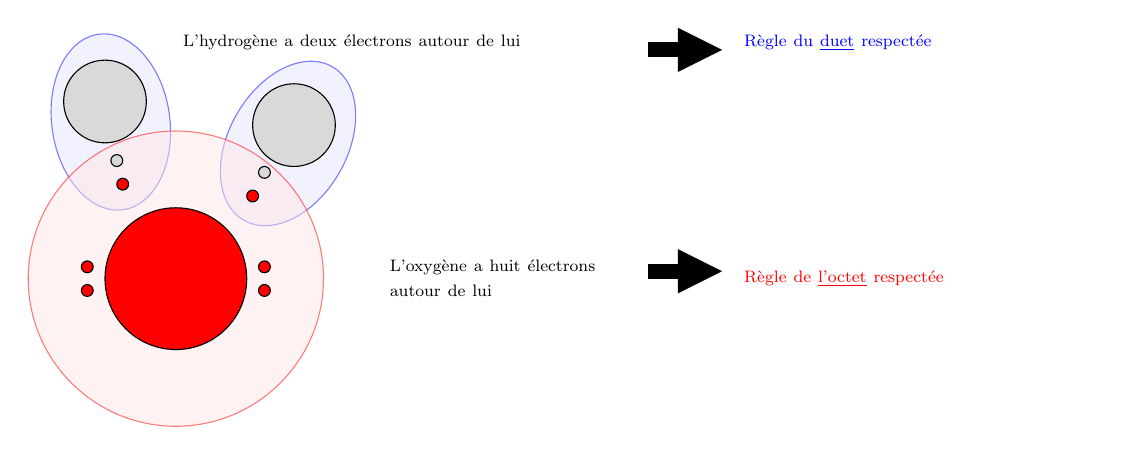
\begin{tikzpicture}[scale=.75, transform shape]
    \fill[blue!10,draw = blue,opacity=.5, rotate = 8] (-1,.8) ellipse(1cm and 1.5cm);
    \fill[blue!10,draw = blue,opacity=.5, rotate = -30] (1.5,1.2) ellipse(1cm and 1.5cm);
    \fill[red!10,draw = red,opacity=.5] (0,-2) circle(2.5);
    
    \fill[red,draw=black] (0,-2) circle(1.2);
    \fill[red,draw=black] (-1.5,-1.8) circle(.1);
    \fill[red,draw=black] (-1.5,-2.2) circle(.1);
    \fill[red,draw=black] (1.5,-1.8) circle(.1);
    \fill[red,draw=black] (1.5,-2.2) circle(.1);
    
    \fill[red,draw=black] (1.3,-.6) circle(.1);
    \fill[red,draw=black] (-.9,-.4) circle(.1);
    
    \fill[gray!30,draw=black] (-1.2,1) circle(.7);
    \fill[gray!30,draw=black] (-1,0) circle(.1);

    \fill[gray!30,draw=black] (2,.6) circle(.7);
    \fill[gray!30,draw=black] (1.5,-.2) circle(.1);

    \pause
    \node[right,text width = 7 cm] (H) at (0,2){\footnotesize L'hydrogène a deux électrons autour de lui};
    \node[right,text width = 4 cm] (O) at (3.5,-2){\footnotesize L'oxygène a huit électrons autour de lui};

    \pause
    \fill[black] (8,2)--(8,1.75)--(9,1.75)--(9,2)--cycle;
    \fill[black] (8.5,1.5)--(8.5,2.25)--(9.25,1.875)--cycle;
    \fill[black] (8,-2)--(8,-1.75)--(9,-1.75)--(9,-2)--cycle;
    \fill[black] (8.5,-1.5)--(8.5,-2.25)--(9.25,-1.875)--cycle;

    \node[right,text width = 6 cm,blue] (HH) at (9.5,2){\footnotesize Règle du \underline{duet} respectée};

    \node[right,text width = 6 cm,red] (OO) at (9.5,-2){\footnotesize Règle de \underline{l'octet} respectée};
    
    \end{tikzpicture}\\ 
    \footnotesize \textbf{Les électrons partagés se déplacent autour des deux atomes.}
\end{frame}

\begin{frame}
\centering
    \begin{figure}
    Comment représenter les molécules pour avoir toutes ces informations sur les électrons de valence et les liaisons formées ?\\
    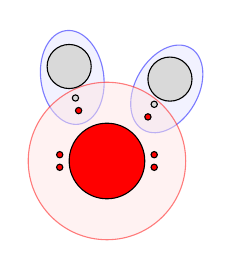
\begin{tikzpicture}[scale=.4, transform shape]
    \fill[blue!10,draw = blue,opacity=.5, rotate = 8] (-1,.8) ellipse(1cm and 1.5cm);
    \fill[blue!10,draw = blue,opacity=.5, rotate = -30] (1.5,1.2) ellipse(1cm and 1.5cm);
    \fill[red!10,draw = red,opacity=.5] (0,-2) circle(2.5);
    
    \fill[red,draw=black] (0,-2) circle(1.2);
    \fill[red,draw=black] (-1.5,-1.8) circle(.1);
    \fill[red,draw=black] (-1.5,-2.2) circle(.1);
    \fill[red,draw=black] (1.5,-1.8) circle(.1);
    \fill[red,draw=black] (1.5,-2.2) circle(.1);
    
    \fill[red,draw=black] (1.3,-.6) circle(.1);
    \fill[red,draw=black] (-.9,-.4) circle(.1);
    
    \fill[gray!30,draw=black] (-1.2,1) circle(.7);
    \fill[gray!30,draw=black] (-1,0) circle(.1);

    \fill[gray!30,draw=black] (2,.6) circle(.7);
    \fill[gray!30,draw=black] (1.5,-.2) circle(.1);
\end{tikzpicture}
    \end{figure}
\end{frame}

\begin{frame}{Représentation de Lewis}

\begin{minipage}{.6\linewidth}
\small
    \begin{itemize}
        \item Les atomes sont représentés par leurs symboles chimiques.
    \end{itemize}
\end{minipage}
\begin{minipage}{.3\linewidth}
\centering
    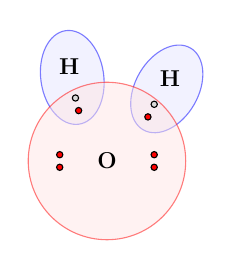
\begin{tikzpicture}[scale=.4, transform shape]
    \fill[blue!10,draw = blue,opacity=.5, rotate = 8] (-1,.8) ellipse(1cm and 1.5cm);
    \fill[blue!10,draw = blue,opacity=.5, rotate = -30] (1.5,1.2) ellipse(1cm and 1.5cm);
    \fill[red!10,draw = red,opacity=.5] (0,-2) circle(2.5);
    
    \node at (0,-2){\huge \textbf{O}};
    \fill[red,draw=black] (-1.5,-1.8) circle(.1);
    \fill[red,draw=black] (-1.5,-2.2) circle(.1);
    \fill[red,draw=black] (1.5,-1.8) circle(.1);
    \fill[red,draw=black] (1.5,-2.2) circle(.1);
    
    \fill[red,draw=black] (1.3,-.6) circle(.1);
    \fill[red,draw=black] (-.9,-.4) circle(.1);
    
    \node at (-1.2,1) {\huge \textbf{H}};
    \fill[gray!30,draw=black] (-1,0) circle(.1);

    \node at (2,.6) {\huge \textbf{H}};
    \fill[gray!30,draw=black] (1.5,-.2) circle(.1);
\end{tikzpicture}
\end{minipage}
\end{frame}

\begin{frame}
\begin{minipage}{.6\linewidth}
\small
    \begin{itemize}
        \item Les atomes sont représentés par leurs symboles chimiques.
        \item Les électrons partagés entre deux atomes dont représentés apr des tirets reliant ces atomes, ils forment une \textcolor{orange}{\textbf{liaison covalente}}.
    \end{itemize}
\end{minipage}
\begin{minipage}{.3\linewidth}
\centering
    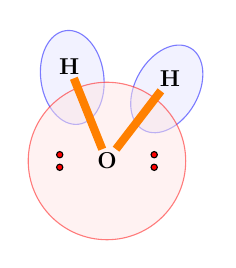
\begin{tikzpicture}[scale=.4, transform shape]
    \fill[blue!10,draw = blue,opacity=.5, rotate = 8] (-1,.8) ellipse(1cm and 1.5cm);
    \fill[blue!10,draw = blue,opacity=.5, rotate = -30] (1.5,1.2) ellipse(1cm and 1.5cm);
    \fill[red!10,draw = red,opacity=.5] (0,-2) circle(2.5);
    
    \node (O) at (0,-2){\huge \textbf{O}};
    \node (HA) at (-1.2,1) {\huge \textbf{H}};
    \node (HB) at (2,.6) {\huge \textbf{H}};
    \draw[line width = 3pt, orange] (HA) -- (O); 
    \draw[line width = 3pt, orange] (HB) -- (O);
    \fill[red,draw=black] (-1.5,-1.8) circle(.1);
    \fill[red,draw=black] (-1.5,-2.2) circle(.1);
    \fill[red,draw=black] (1.5,-1.8) circle(.1);
    \fill[red,draw=black] (1.5,-2.2) circle(.1);
\end{tikzpicture}
\end{minipage}
\end{frame}

\begin{frame}
\begin{minipage}{.6\linewidth}
\small
    \begin{itemize}
        \item Les atomes sont représentés par leurs symboles chimiques.
        \item Les électrons partagés entre deux atomes dont représentés apr des tirets reliant ces atomes, ils forment une \textcolor{orange}{\textbf{liaison covalente}}.
        \item Les électrons de valence qui ne forment pas de liaison sont représentés apr des tirets (1 tiret = 2 électrons), appelés \textcolor{olive}{\textbf{doublets non liants}}.
    \end{itemize}
\end{minipage}
\begin{minipage}{.3\linewidth}
\centering
    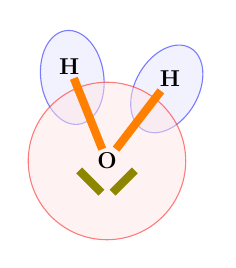
\begin{tikzpicture}[scale=.4, transform shape]
    \fill[blue!10,draw = blue,opacity=.5, rotate = 8] (-1,.8) ellipse(1cm and 1.5cm);
    \fill[blue!10,draw = blue,opacity=.5, rotate = -30] (1.5,1.2) ellipse(1cm and 1.5cm);
    \fill[red!10,draw = red,opacity=.5] (0,-2) circle(2.5);
    
    \node (O) at (0,-2){\huge \textbf{O}};
    \node (HA) at (-1.2,1) {\huge \textbf{H}};
    \node (HB) at (2,.6) {\huge \textbf{H}};
    \draw[line width = 3pt, orange] (HA) -- (O); 
    \draw[line width = 3pt, orange] (HB) -- (O);
    \draw[line width = 3pt,olive,rotate = 45] (-2,-2.25)--(-1,-2.25);
    \draw[line width = 3pt,olive,rotate = -45] (1,-2.25)--(2,-2.25);
\end{tikzpicture}
\end{minipage}
\end{frame}

%%%%%%%%%%%%%%%%%%%%%%%%%%%%%%%%%%%%%
\end{document}